\documentclass[letterpaper]{article}
\usepackage[margin=1in]{geometry}
\usepackage[utf8]{inputenc}
\usepackage{textcomp}
\usepackage{amssymb}
\usepackage{natbib}
\usepackage{graphicx}
\usepackage{gensymb}
\usepackage{amsthm, amsmath, mathtools}
\usepackage[dvipsnames]{xcolor}
\usepackage{enumerate}
\usepackage{mdframed}
\usepackage[most]{tcolorbox}
\usepackage{csquotes}
% https://tex.stackexchange.com/questions/13506/how-to-continue-the-framed-text-box-on-multiple-pages

\tcbuselibrary{theorems}

\newcommand{\R}{\mathbb{R}}
\newcommand{\Z}{\mathbb{Z}}
\newcommand{\N}{\mathbb{N}}
\newcommand{\Q}{\mathbb{Q}}
\newcommand{\C}{\mathbb{C}}
\newcommand{\code}[1]{\texttt{#1}}
\newcommand{\mdiamond}{$\diamondsuit$}
\newcommand{\PowerSet}{\mathcal{P}}
\newcommand{\Mod}[1]{\ (\mathrm{mod}\ #1)}
\DeclareMathOperator{\lcm}{lcm}

%\newtheorem*{theorem}{Theorem}
%\newtheorem*{definition}{Definition}
%\newtheorem*{corollary}{Corollary}
%\newtheorem*{lemma}{Lemma}
\newtheorem*{proposition}{Proposition}


\newtcbtheorem[number within=section]{theorem}{Theorem}
{colback=green!5,colframe=green!35!black,fonttitle=\bfseries}{th}

\newtcbtheorem[number within=section]{definition}{Definition}
{colback=blue!5,colframe=blue!35!black,fonttitle=\bfseries}{def}

\newtcbtheorem[number within=section]{corollary}{Corollary}
{colback=yellow!5,colframe=yellow!35!black,fonttitle=\bfseries}{cor}

\newtcbtheorem[number within=section]{lemma}{Lemma}
{colback=red!5,colframe=red!35!black,fonttitle=\bfseries}{lem}

\newtcbtheorem[number within=section]{example}{Example}
{colback=white!5,colframe=white!35!black,fonttitle=\bfseries}{def}

\newtcbtheorem[number within=section]{note}{Important Note}{
        enhanced,
        sharp corners,
        attach boxed title to top left={
            xshift=-1mm,
            yshift=-5mm,
            yshifttext=-1mm
        },
        top=1.5em,
        colback=white,
        colframe=black,
        fonttitle=\bfseries,
        boxed title style={
            sharp corners,
            size=small,
            colback=red!75!black,
            colframe=red!75!black,
        } 
    }{impnote}
\usepackage[utf8]{inputenc}
\usepackage[english]{babel}
\usepackage{fancyhdr}
\usepackage[hidelinks]{hyperref}

\pagestyle{fancy}
\fancyhf{}
\rhead{Math 170B}
\chead{Monday, April 24, 2023}
\lhead{Lecture 10}
\rfoot{\thepage}

\setlength{\parindent}{0pt}

\begin{document}

\section{Polynomial Interpolation (Section 6.1)}
Suppose we're given $m + 1$ data points, 
\[(x_i, y_i), \quad 0 \leq i \leq m,\]
and we want to seek a polynomial $P$ of the \emph{lowest possible degree} for which \[P(x_i) = y_i, \quad 0 \leq i \leq m.\] Such a polynomial $P$ is said to \textbf{interpolate} the data. 

\begin{mdframed}
    (Example.) Suppose we have the following data points.
    \begin{center}
        \begin{tabular}{c|c c c c}
            $x$ & -5 & -3 & -1 \\
            \hline  
            $y$ & 0 & -2 & 0
        \end{tabular}
    \end{center}
    Drawing the points and the associated curve, 
    \begin{center}
        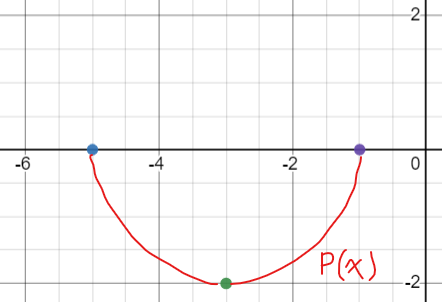
\includegraphics[scale=0.5]{../assets/interpolation_ex1.png}
    \end{center}
    schematically, we can represent the data points above with the polynomial 
    \[P(x) = \frac{1}{2}\left(x + 3\right)^{2} - 2.\]
    We don't care about what the curve looks like beyond those points. The interpolation condition just ensures that the curve associated with the polynomial goes through the \emph{given} points. 
\end{mdframed}
\textbf{Remarks:}
\begin{itemize}
    \item If we were just given a single point, then the lowest-degree polynomial we can create is a constant polynomial, $P(x) = y_0$. 
    \item If we had two points, then we can draw a line through the points and the lowest-degree polynomial we can create is a linear equation. 
\end{itemize}

The theorem that governs this problem is shown below. 
\begin{theorem}{Polynomial Interpolation}{}
    If $x_0, x_1, \hdots, x_m$ are distinct real numbers, then for arbitrary values $y_0, y_1, \hdots, y_m$, there exists a \underline{unique} polynomial $P_{m}$ of degree \underline{at most} $m$ such that \[P_{m}(x_i) = y_i \quad (0 \leq i \leq m)\]
\end{theorem}

\begin{proof}
    We'll show both aspects of the theorem. 
    \begin{itemize}
        \item \underline{Uniqueness:} Suppose we have two interpolating polynomials $P_{m}(x_i) = y_i$ and $Q_{m}(x_i) = y_i$, both of which are degree $m$. Then, their difference, $P_{m}(x) - Q_{m}(x)$, also has at most degree $m$. This means that this difference polynomial has at most $m$ zeros/roots. But, as both $P_m$ and $Q_m$ are interpolating polynomials, $P_{m}(x_i) - Q_{m}(x_i) = y_i - y_i = 0$ has $m + 1$ zeros. Thus, $P_m(x) - Q_m(x) = 0$ has zeros everywhere and thus $P_m(x) = Q_m(x)$. 
        \item \underline{Existence:} Suppose, for $k \geq 1$, $P_{k - 1}(x)$ has degree $k - 1$. In other words, $P_{k - 1}(x_i) = y_i$ for $0 \leq i \leq k - 1$. Suppose we want to construct the next higher-degree polynomial, degree $k$, such that $P_{k}(x_i) = y_i$ for $0 \leq i \leq k$. Then, \[P_{k}(x) = P_{k - 1}(x) + c(x - x_0)(x - x_1) \hdots (x - x_{k - 1}).\] 
        Then, \[P_{k}(x_i) = P_{k - 1}(x_i) + c \cdot 0 = P_{k - 1}(x_i) = y_i, \quad (0 \leq i \leq k - 1).\]
        So, set $P_{k}(x_k) = y_k$ and then solve for $c$. More specifically, 
        \[P_{k}(x_k) = y_k = P_{k - 1}(x_k) + c(x_k - x_0)(x_k - x_1)(x_k - x_2) \hdots (x_k - x_{k - 1}).\]
        By solving for $c$, we have 
        \[c = \frac{y_k - P_{k - 1}(x_k)}{(x_k - x_0)(x_k - x_1)(x_k - x_2) \hdots (x_k - x_{k - 1})}.\]
    \end{itemize}
    This concludes the proof.
\end{proof}

\subsection{Polynomial Representation}
There are different ways we can represent these polynomials, although keep in mind that they all represent the same function. 

\subsubsection{Newton's Form}
Newton's Form is
\begin{equation}
    P_{m}(x) = c_0 + c_1 (x - x_0) + c_2 (x - x_0)(x - x_1) + \hdots + c_m (x - x_0)(x - x_1) \hdots (x - x_{m - 1})
\end{equation}
Note that this form models $m + 1$ data points $(0 \leq i \leq m)$. Notice, however, that we never include $x_m$ in our final equation. The first few cases of the above equation are 
\[\begin{aligned}
    P_{0}(x) &= c_0 \\ 
    P_{1}(x) &= c_0 + c_1 (x - x_0) \\ 
    P_{2}(x) &= c_0 + c_1 (x - x_0) + c_2 (x - x_0) (x - x_1)
\end{aligned}\]

\begin{mdframed}
    (Example.) Suppose we have the polynomial $P_{m}(t)$, for $t \in \R$ (i.e., we're evaluating this polynomial with value $t$). We can write an algorithm similar to Horner's method for evaluating this polynomial. Then, we'll have the inputs $x_i$, $c_i$ for $0 \leq i \leq m$, and $t \in \R$. 
    \begin{algorithm}[H]
        \caption{Finding the Polynomial}
        \label{alg:two}
        \begin{algorithmic}[1]
            \State $p \gets c_m$
            \For{$k \gets m - 1$ to $0$ step $-1$}
                \State $p \gets (t - x_k) \cdot p + c_k$
            \EndFor 
        \end{algorithmic}
    \end{algorithm}
\end{mdframed}
To find the coefficients $c_k$, we have 
\begin{equation}
    c_k = \begin{cases}
        y_0 & k = 0 \\ 
        \frac{y_k - P_{k - 1}(x_k)}{(x_k - x_0)(x_k - x_1)(x_k - x_2) \hdots (x_k - x_{k - 1})} & k \geq 1
    \end{cases}.
\end{equation}
To compute the coefficients, we can make use of the following algorithm. Given 
\begin{itemize}
    \item $x_i \quad (0 \leq i \leq m)$
    \item $y_i \quad (0 \leq i \leq m)$
\end{itemize}
this algorithm should output $c_i$ for $0 \leq i \leq m$. 
\begin{algorithm}[H]
    \caption{Computing $c_i$}
    \begin{algorithmic}[1]
        \State $c_0 \gets y_0$
        \For{$k \gets 1$ to $m$}
            \State $d \gets (x_k - x_{k - 1})$
            \State $p \gets c_{k - 1}$
            \For{$i \gets k - 2$ to $0$ step $-1$}
                \State $d \gets d(x_k - x_i)$ \Comment{Denominator}
                \State $p \gets p(x_k - x_i) + c_i$ \Comment{$P_{k - 1}(x_k)$} 
            \EndFor 
            \State $c_k \gets (y_k - p) / d$
        \EndFor 
    \end{algorithmic}
\end{algorithm}


\begin{mdframed}
    (Example.) Suppose we have the data points 
    \begin{center}
        \begin{tabular}{c|c c c c}
            $x$ & 5 & -7 & -6 & 0 \\ 
            \hline 
            $y$ & 1 & -23 & -54 & -954 
        \end{tabular}
    \end{center}
    Newton's form for the polynomial looks like 
    \[P(x) = c_0 + c_1 (x - 5) + c_2 (x - 5)(x + 7) + c_3 (x - 5)(x + 7)(x + 6).\]
    Then, we can compute each of the $c_i$ for $0 \leq i \leq m = 3$. 
    \begin{itemize}
        \item $i = 0$: we know that 
        \[c_0 = y_0 = 1.\]

        \item $i = 1$: we have 
        \[c_1 = \frac{y_1 - P_{0}(x_1)}{(x_1 - x_0)} = \frac{-23 - 1}{(-7 - 5)} = 2.\]

        \item $i = 2$: we have
        \[c_2 = \frac{y_2 - P_{1}(x_2)}{(x_2 - x_0) (x_2 - x_1)} = \frac{-54 - (c_0 + c_1 (x_2 - x_0))}{(-6 - 5)(-6 - (-7))} = \frac{-54 - (1 + 2(-6 - 5))}{(-6 - 5)(-6 - (-7))} = 3.\]

        \item $i = 3$: by the same process as above, we find that $c_3 = 4$.
    \end{itemize}
\end{mdframed}


\end{document}